\begin{frame}{Relational Properties}

    A property that relates multiple executions of (the same or different) program(s) is referred to as a \textit{relational property}.
    \pause
    \vspace{20pt}
    \begin{tcolorbox}[
        colback=white,
        colframe=green,
        colbacktitle=white!70!green,
        coltitle=black,
        title=\textbf{Hoare Triple.},
        enhanced,
        attach boxed title to top left={yshift=-2mm, xshift=0.5cm},%
        ]
        \[
        \colorbox{yellow!20!white}{\{\textsc{Pre}($\vec{x}$)\}}\ \prog\ \colorbox{green!20!white}{\{\textsc{Post}($y$)\}}
        \]
    \end{tcolorbox}
    \pause
    \begin{tcolorbox}[
        colback=white,
        colframe=blue,
        colbacktitle=white!70!blue,
        coltitle=black,
        title=\textbf{Relational Property as a Hoare Triple.},
        enhanced,
        attach boxed title to top left={yshift=-2mm, xshift=0.5cm},%
        ]
        \[
        \colorbox{yellow!20!white}{\{\textsc{Pre}($\vec{x_1}$, $\vec{x_2}$)\}}\ \prog_1, \prog_2\ \colorbox{green!20!white}{\{\textsc{Post}($y_1$, $y_2$)\}}
        \]
    \end{tcolorbox}

    \pause
    \vspace{20pt}

    When both programs $\prog_1$ and $\prog_2$ are the same programs, i.e \prog, \textit{relational properties} become
    \textbf{hyper-properties}!.
\end{frame}

\begin{frame}[fragile]{What is program sketching?}
    A partial program (referred to as a \textit{sketch}), which leaves out certain \boxed{holes} for the synthesizer to fill such that the completed program satisfies the required specification.
    \pause
    \vspace{10pt}
    \begin{figure}
        \begin{minipage}{0.48\columnwidth}
            \centering
            Specification as a \textbf{Hoare Triple}, $\{P\}Q\{R\}$
            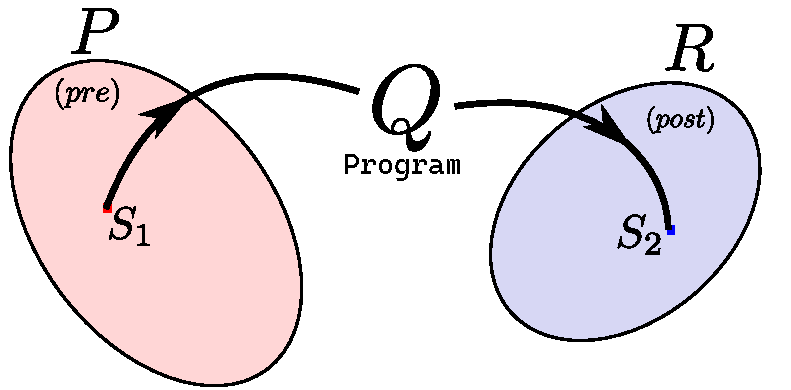
\includegraphics[scale=0.35]{assets/hoare_triple.pdf}
        \end{minipage}
        \hfill
        \pause
        \begin{minipage}{0.5\columnwidth}
            \begin{minted}{c}
                int |$\prog$|(int n){
                    // |$PRE:$ \colorbox{yellow!20!white}{assume(n > 1);}|
                    int i = 0, x = 0;
                    while(i < n){
                        i = i + 1;
                        x = |\boxed{\cdot}|
                    }
                    // |$POST:$ \colorbox{green!10!white}{assert(x > 2 * n);}|
                    return x;
                }
            \end{minted}
        \end{minipage}

    \end{figure}
\end{frame}

\begin{frame}{Lifting Program Sketching to Relational Sketching}

    Given partial programs $\proghole{1}{\cdot}$ and $\proghole{2}{\cdot}$, find completion $\E$, where $\E.H$ and $\E.G$ respective completions of $\proghole{1}{\cdot}$ and $\proghole{2}{\cdot}$ that satisfy a specification.
    \pause
    \vspace{20pt}
    \begin{tcolorbox}[
        colback=white,
        colframe=green,
        colbacktitle=white!70!green,
        coltitle=black,
        title=\textbf{Relational Synthesis},
        enhanced,
        attach boxed title to top left={yshift=-2mm, xshift=0.5cm},%
        ]
        \[ \exists \E. \ \colorbox{yellow!20!white}{\{\textsc{Pre}($\vec{x_1}$, $\vec{x_2}$)\}}\ \proghole{1}{\E.H}, \proghole{2}{\E.G}\ \colorbox{green!20!white}{\{\textsc{Post}($y_1$, $y_2$)\}}
        \]
    \end{tcolorbox}
\end{frame}